\documentclass [border = .2cm] {standalone}

% Required packages
\usepackage{pgfplots}
\pgfplotsset{compat = newest}
\usetikzlibrary {backgrounds}

\begin{document}
	
	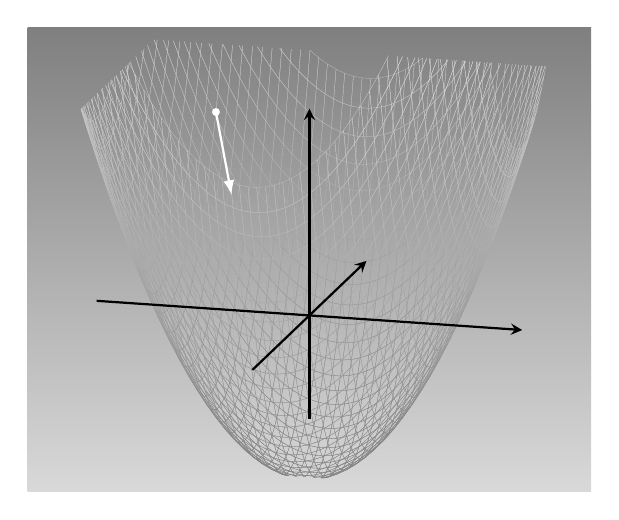
\begin{tikzpicture}		
		[background rectangle/.style=
		{bottom color=white!70!gray!},
		show background rectangle]
		
		\begin{axis}[
			 view = {15}{20},
			 colormap={blackwhite}{gray(0cm)=(0.5); gray(1cm)=(1)},
			 thick,
			 axis lines = center,
			 axis on top,
			 color=black,
			 xmax = 10,
			 xmin = -10,
			 ymax = 10, 
			 ymin = -10, 
			 zmax = 12, 
			 zmin = -6,
			 xticklabels=\empty,
			 yticklabels=\empty,
			 zticklabels=\empty,
			 xtick=false,
			 ytick=false,
			 ztick=false,
			 ]
			
			\addplot3 [
			domain=-10:10,
			domain y = -10:10,
			samples = 50,
			samples y = 50,
			surf,
			mesh,
			ultra thin,
			shader = interp,
			no marks,
			] {0.2 * x^2 + 0.2 * y^2 - 9.4};
			
		
		
		\coordinate (A) at (-6,6,9.4);
		\coordinate (B) at (-5,5,5);
		
		\draw [fill=white, white] (A) circle (1pt) node [left] {};
		
		\draw [-latex, white, thick] (A) -- (B);
		
				
		\end{axis}
		
	\end{tikzpicture}
	
\end{document}